
\section{Question Answering}


\begin{frame}{Question Answering - Introduction }
An application of short Post-Response is Question Answering system, such as IBM Watson (Jeopardy).
In this case most of the candidate responses are answers for factoid questions
\begin{itemize}
	\item Open domain  question  answering  has become important research area in natural language processing
	\item Tougher than  common  search  engine  tasks
	\begin{itemize}
		\item Finding accurate and concise answers  to  questions rather  than  a  set of relevant  document
	\end{itemize}
	\item Simple term-based retrieval won't be enough
	\item \textbf{Type} of the sought after answer should be known to retrieve accurate answers
\end{itemize}

\end{frame}

\begin{frame}[fragile,shrink]{Question Answering - Samples}
	\begin{tabular}{p{8cm}|p{3cm}|p{3cm}}
		Question&Hierarchy&Type\\
		\hline
		What is RNN?&Abbreviation&Expansion\\
		Where is the big temple in India located?&Location&City\\
		Who was the president of India in 2006?&Human&Person\\
		Name the currency used in China&Entity&Currency\\
		How far away is the moon?&Numeric&Distance\\
		What is the chemical symbol for oxygen?&Entity&Symbol\\
		What is a prism?&Description&Definition\\
		Why is the sun yellow?&Description&Reason\\
		When did CV Raman receive his Nobel Prize?&Numeric&Year\\
		\hline
	\end{tabular}\\
Most questions could be classified in to 6 major classes\footnote{Xin Li, Dan Roth, Learning Question Classifiers} - ABBREVIATION, ENTITY,DESCRIPTION, HUMAN,  LOCATION and  NUMERIC VALUE and around 50 fine-grained types.
\end{frame}

\begin{frame}[fragile,shrink=20]{Definition of Question classes}
    \begin{minipage}[t]{0.49\linewidth}
    \begin{tabular}{|>{\raggedright\arraybackslash}m{3cm}|>{\raggedright\arraybackslash}m{3cm}|}
        \hline
        \textbf{Class}   & \textbf{Definition} \\
        \hline
        ABBREVIATION & abbreviation \\
        \hline
        abb & abbreviation \\
        \hline
        exp & expression abbreviated \\
        \hline
        ENTITY & entities \\
        \hline
        animal & animals \\
        \hline
        body & organs of body \\
        \hline
        color & colors \\
        \hline
        currency & currency names \\
        \hline
        dis.med. & diseases and medicine \\
        \hline
        LOCATION & locations \\
        \hline
        city & cities \\
        \hline
        country & countries \\
        \hline
        mountain & mountains \\
        \hline
        $\cdots$ & $\cdots$ \\
        \hline
    \end{tabular}
    \end{minipage}
    \begin{minipage}[t]{0.49\linewidth}
       \begin{tabular}{|>{\raggedright\arraybackslash}m{3cm}|>{\raggedright\arraybackslash}m{3cm}|}
           \hline
           NUMERIC & numeric values \\
           \hline
           code & postcodes or other codes \\
           \hline
           date & dates \\
           \hline
           DESCRIPTION & description and abstract concepts  \\
           \hline
           definition & definition of sth. \\
           \hline
           $\cdots$ & $\cdots$  \\
           \hline
           HUMAN & human beings  \\
           \hline
           group & a group or organization of persons  \\
           \hline
           ind & an individual \\
           \hline
           title & title of a person \\
           \hline
           description & description of a person \\
           \hline
           $\cdots$&$\cdots$\\
           \hline
       \end{tabular}
    \end{minipage}
    Reference: \href{https://cogcomp.seas.upenn.edu/Data/QA/QC/definition.html}{Definition of Question Classes}
\end{frame}

\begin{frame}[fragile, shrink]{Experimental Data for Question Classification}
    \small
    \begin{verbatim}
        ENTY:cremat What films featured the character Popeye Doyle ?
        ENTY:animal What fowl grabs the spotlight after
                    the Chinese Year of the Monkey ?
        ABBR:exp What is the full form of .com ?
        LOC:city What city did the Flintstones live in ?
        LOC:other Where is the Kalahari desert ?
        HUM:gr What company tabulates the ballots in
                   voting for the Academy Awards ?
        DESC:desc What do Mormons believe ?
        NUM:money How much money does a back injury lawsuit get ?
        NUM:other What was Einstein's IQ ?
        NUM:count How many people died on D-Day ?
        ABBR:exp What does 'PSI' stand for ?
        ...
    \end{verbatim}
    Reference: \href{https://cogcomp.seas.upenn.edu/Data/QA/QC/}{Training Data for Text Retrieval Conference (TREC)}
\end{frame}

\begin{frame}[fragile, shrink=10]{Feature Space}
    \begin{multicols}{2}
        \begin{itemize}
            \item Words
            \item Part of Speech (POS) tags
            \item Chunks(non-overlapping phrases)
            \item Named entities
            \item Head  chunks(using POS - first  noun  chunk\footnote{In English grammar, a head is the key word that determines the nature of a phrase}  in  a  sentence)\footnote{A trip to Cape Carnival, FL, takes 10 hours. The distance is 816 km. Calculate the average speed}
            \item Semantically  related  words (words  that often occur with a specific question class - How far, How high, How long)
        \end{itemize}
            \end{multicols}
            Contiguous chinking - Example
             \begin{center}
                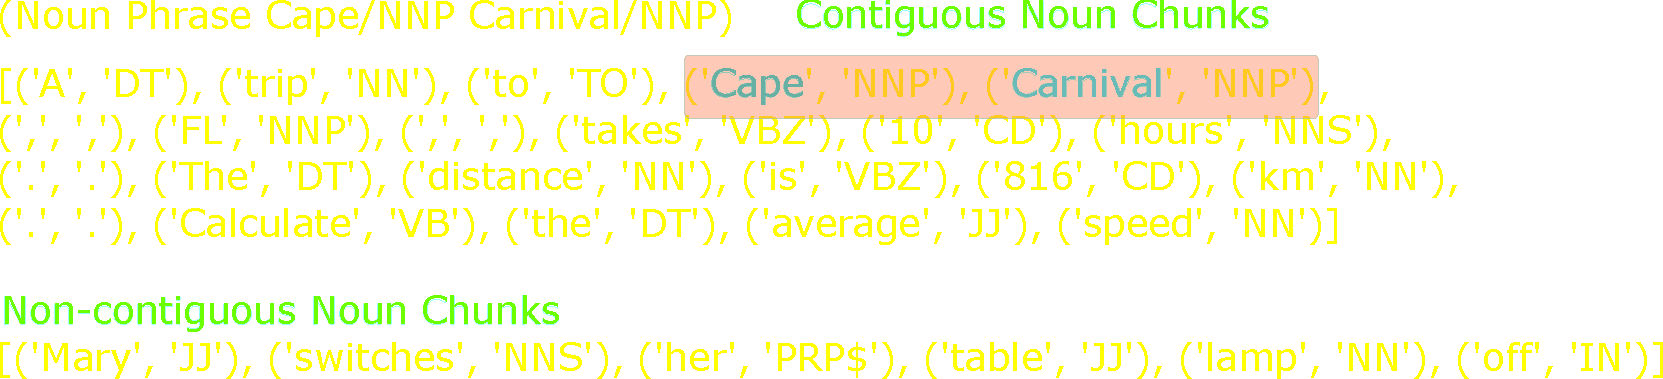
\includegraphics[width=0.85\linewidth]{./Images/POS}
            \end{center}
            \begin{description}
                \item[Non-contiguous phrase example] Mary switches her table lamp off
            \end{description}
\end{frame}
\begin{frame}[fragile,shrink=9]{Chunking using NLTK}
\begin{lstlisting}
import nltk
from nltk.tokenize import word_tokenize
from nltk import word_tokenize, pos_tag

def regex_chunker(text, regex):

    sent = pos_tag(word_tokenize(text))
    cp = nltk.RegexpParser(regex)
    chunked_pos_tags = cp.parse(sent)

    for chunk in chunked_pos_tags.subtrees(
                    filter=lambda t: t.label() == 'Noun Phrase'):
        print(chunk)

if __name__ == '__main__':
    text = '''A trip to Cape Carnival, FL, takes 10 hours.
                    The distance is 816 km. Calculate the average speed'''
    regex_chunker(text, r'Noun Phrase: {<NN.?>+<NN.?>}')
\end{lstlisting}
\end{frame}

\begin{frame}{Question Typology Rules}
Simple rules could be defined to classify questions\\
For example, \\
\begin{description}
	\item[1.] $if \;QuestionStartsWith(who) \,or\, QuestionStartsWith(whom)$\\
	$\quad TopHierarchy \leftarrow \, \textit{HUMAN}$\\
	$\quad Class \leftarrow \textit{PERSON}$\\
	$fi$
	\item[2.]$if\; QuestionStartsWith(where)$\\
	$\quad TopHierarchy \leftarrow \, \textit{LOCATION}$\\
	$\quad Class \leftarrow \textit{CITY}$\\
	$fi$\\


	\item[]\textit{If  a  query  contains Which or What,  then the  head  noun phrase determines the class, as for What X questions}\\
	What is a prism?
\end{description}
\end{frame}
\begin{frame}{Learning Question Classifiers}
    \begin{minipage}{0.48\linewidth}
        \begin{itemize}
            \item Answering factual questions\cite{li-roth-2002-learning}
            \item understanding the question's intent and the type of answer it seeks
            \item Classifying questions into categories
            \item Constraining the search for potential answers
            \item Guide answer verification
        \end{itemize}
    \end{minipage}
    \begin{minipage}{0.48\linewidth}
    \begin{itemize}
        \item Uses lexical features for classification
        \item [] Lexical features include words, phrases, and part-of-speech tags extracted from the question
        \item The authors use a two-layer question taxonomy with coarse-grained (e.g., definition, location) and fine-grained (e.g., person, city) categories
        \item Different machine learning algorithms (Naive-Bayes)can be used using the  labeled question-answer pairs
    \end{itemize}
        \end{minipage}
\end{frame}

\begin{frame}{Learning Question Classifiers}
    \begin{center}
        \begin{figure}
            \includegraphics[width=0.85\linewidth]{"./Images/Learning Question Classifiers"}
        \end{figure}

    \end{center}

\end{frame}

\begin{frame}{Decision Rule}
Given the list of classes and the features for each of the question, it is easy to calculate the probability distribution of classes for the given question\cite{li-roth-2002-learning}\\
The probability density is
\begin{equation}
P = [p_1,p_2,\ldots, p_n]
\end{equation} and the corresponding class labels are \begin{equation}
C= [c_1,c_2,\ldots,c_n]
\end{equation}
$p_i$s are obtained by employing Naive-Bayes algorithm
\end{frame}

\begin{frame}
    \centering
    \Huge{QA Using Neural Models}
\end{frame}

\begin{frame}{Reading Comprehension}
    \Large
    Reading comprehension task seeks to estimate the conditional probability
    \begin{align}
        p(a\mid c, q)
    \end{align}where $c$ is a context document\\
    a query relating to that document, $q$ and \\
    the answer to that query, $a$.
\end{frame}
\begin{frame}{Components of a QA System}
    \begin{figure}
        \centering
        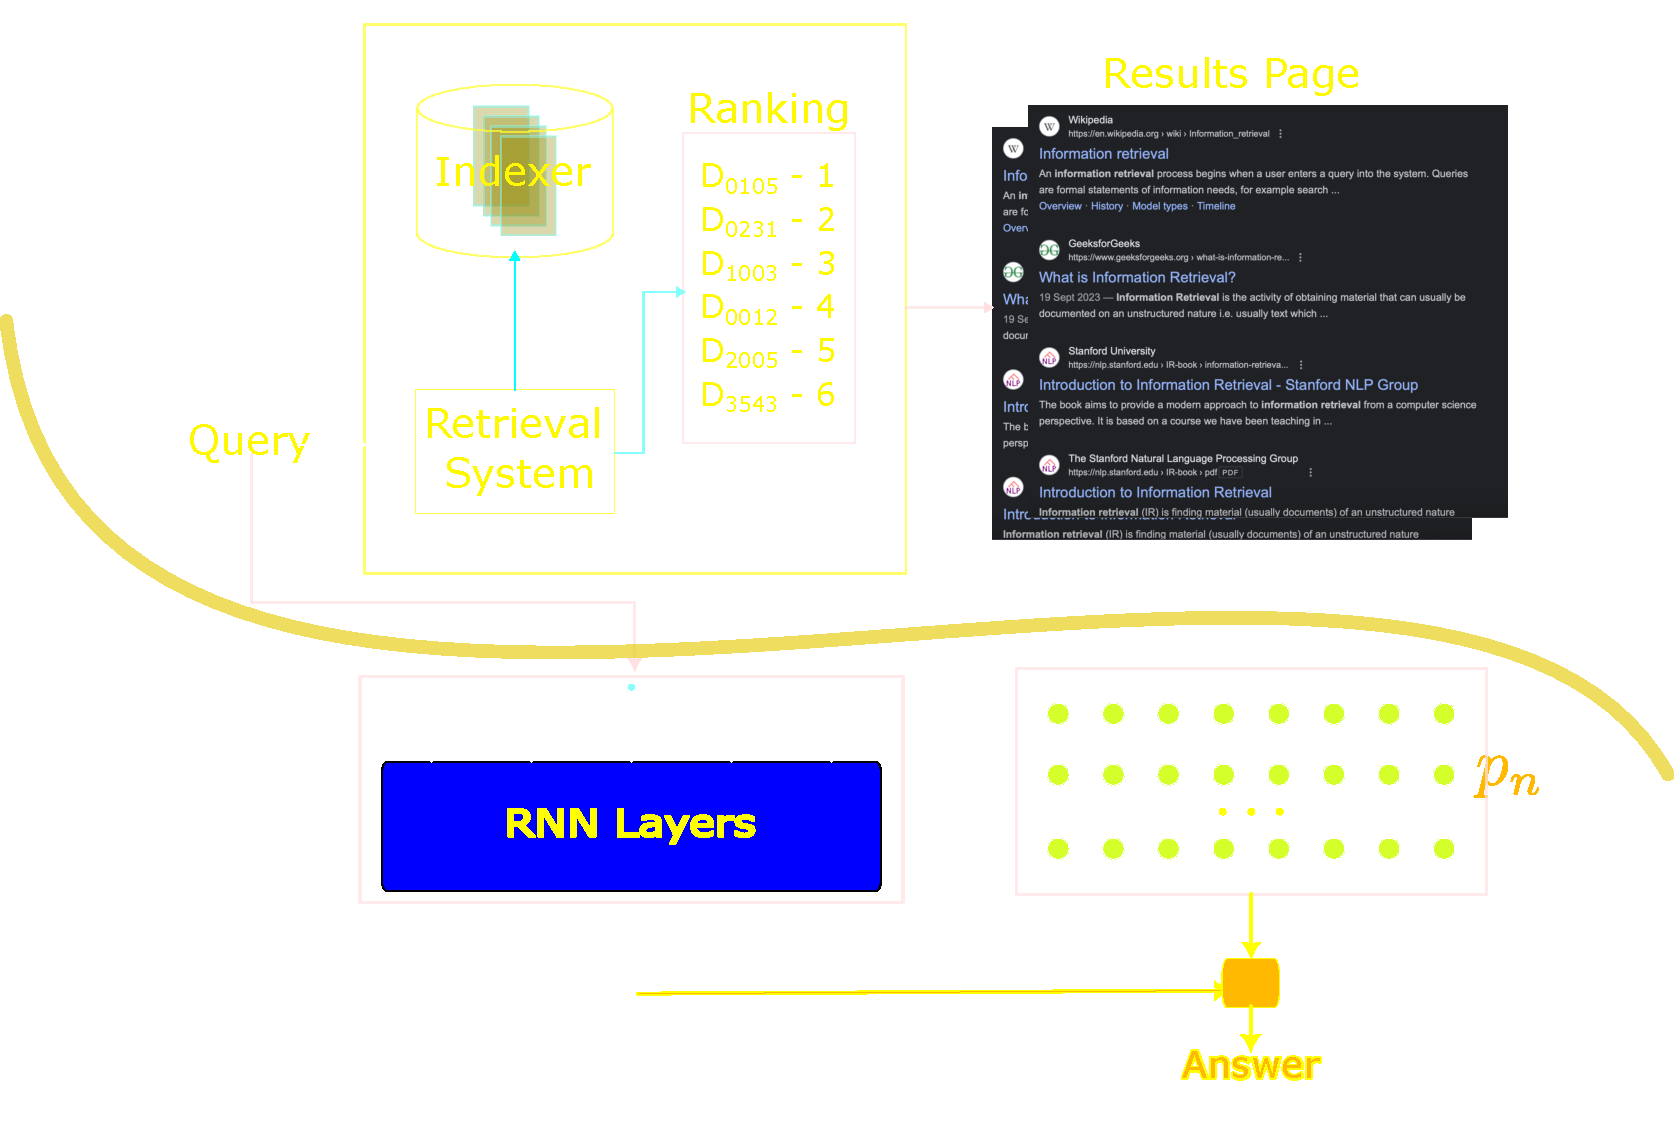
\includegraphics[width=0.7\linewidth]{Images/SimpleRetriever}
        \caption{QA System}
        \label{fig:simpleretriever}
    \end{figure}

\end{frame}
\begin{frame}{Identifying Span of Tokens}
    \begin{minipage}{0.35\linewidth}
        \begin{enumerate}
            \item[] Who is CV Raman?
            %	\item [] What is the invention of CV Raman?
            %	\item [] What is the highest civilian award won by him?
            %	\item [] When did he receive the Nobel prize?
        \end{enumerate}
    \end{minipage}
    \begin{minipage}{0.6\linewidth}

        Sir CV Raman (7 November 1888-21 November 1970) was an \colorbox{yellow!55}{\color{blue}Indian physicist} born in the former Madras Province in India (presently the state of Tamil Nadu), who carried out ground-breaking work in the field of light scattering, which earned him the 1930 Nobel Prize for Physics. He discovered that when light traverses a transparent material, some of the deflected light changes wavelength and amplitude. This phenomenon, subsequently known as Raman scattering, results from the Raman effect[4] In 1954, the Indian government honored him with India's highest civilian award, the Bharat Ratna [5][6]
    \end{minipage}
\end{frame}

\begin{frame}{Identifying Span of Tokens}
    \begin{minipage}{0.35\linewidth}
        \begin{enumerate}
            %\item[] Who is CV Raman?
            \item [] What is the invention of CV Raman?
            %	\item [] What is the highest civilian award won by him?
            %	\item [] When did he receive the Nobel prize?
        \end{enumerate}
    \end{minipage}
    \begin{minipage}{0.6\linewidth}

        Sir CV Raman (7 November 1888-21 November 1970) was an Indian physicist born in the former Madras Province in India (presently the state of Tamil Nadu), who carried out ground-breaking work in the field of light scattering, which earned him the 1930 Nobel Prize for Physics. \colorbox{yellow!35}{\parbox{0.98\textwidth}{\color{blue}He discovered that when light traverses a transparent material, some of the deflected light changes wavelength and amplitude.}} This phenomenon, subsequently known as Raman scattering, results from the Raman effect[4] In 1954, the Indian government honored him with India's highest civilian award, the Bharat Ratna [5][6]
    \end{minipage}
\end{frame}



\begin{frame}[shrink=15]{Answer Extraction}
The important phase $\smile$ in the QA system\\
\textbf{Span Labeling}: The span of text (tokens) that contains the answer. The task of finding the span of text is known as Span Labeling\\

Modern approaches combine a IR-based component   based   on   bigram   hashing and  TF*IDF  matching  and a  multi-layer recurrent neural network model trained to detect  answers \cite{hermann2015teaching} \cite{chen2017reading}
\rule{\linewidth}{0.1mm}
\begin{minipage}{0.4\linewidth}
Emerging systems are designed as reading comprehension systems
\begin{figure}
	\centering
	\includegraphics[width=0.9\linewidth]{./Images/AnswerProcessing}
	\label{fig:answerprocessing}
\end{figure}
\end{minipage}
\begin{minipage}{0.59\linewidth}
    Two important components
\begin{itemize}
    \item \textbf{Document Retriever}: Utilizes bigram hashing and TF-IDF matching to efficiently return relevant articles based on a given question.
    \item \textbf{Document Reader}: A multi-layer recurrent neural network model trained to extract answer spans from the retrieved documents.
\end{itemize}
\end{minipage}
\rule{\linewidth}{0.1mm}

\end{frame}

\begin{frame}{Document Retriever}
\begin{itemize}
	\item Using a typical Term-Document and the retrieval operations on the Term-Document matrix
	\item Using Inverted Indexing approach used in SOLR/Elastic search
	\item Using LSA
	\item Combination of the above with n-grams
	\item Using a ranking model to retrieve top 5-10 documents
	\item Use an answer encoder to find similar representations in the documents - Use of RNN
\end{itemize}
\end{frame}


\begin{frame}{Features for Answers }
\begin{itemize}
	\item Phrase matches keywords/patterns of question and the paragraph
	\item Count of terms that match question and potential paragraphs
	\item Cosine similarity
	\item Pattern matching using trained ANNs
	\item Probabilistic methods using alignment methods
\end{itemize}
\end{frame}

\begin{frame}{Question Encoding}
\begin{itemize}
	\item A question encoder creates weighted sum of all the words ($q_i$) in a question.
	\item 	The word embedding of each word in the question is fed to an RNN encoder
	\item For every time state, $q_i$, a hidden $\mathbf{q}_i$ is output from the hidden unit.
	\item For all the time states, a weighted sum $\mathbf{q}$ and a single embedding of the question is the output - $\mathbf{q} = \left[\mathbf{q}_1,\mathbf{q}_2,\mathbf{q}_3,\ldots\mathbf{q}_l\right]$

\end{itemize}
\begin{align}
\mathbf{q} &= \sum_j b_jq_j \\
b_j &= \dfrac{\exp({\textbf{w}}.\textbf{q}_j)}{\sum_{i}^{t}\exp(\textbf{w}.\textbf{q}_i)}
\end{align}
where $\textbf{w}$ is the weight vector to be learned
\end{frame}


\begin{frame}{Paragraph Encoding}
Let $q = (q_1,q_2,\ldots, q_n)$ be the question with $n$ tokens\\
Let $\mathbf{p} = (\mathbf{p_1},\mathbf{p_2},\dots, \mathbf{p_m})$ be the encoded paragraphs of $\hat{p} = (\hat{p}_1,\hat{p}_2,\ldots, \hat{p}_m)$\\
and $\hat{p}_i$ represent the following:
\begin{enumerate}
	\item The embedding of the word $f_1 = E(p_i)$
	\item $p_i$ can be matched exactly by one question word $f_2 = \mathfrak{1} (p_i \in q_i)$
	\item Token feature such as POS, NER, TF/TF*IDF - $f_{features}$
	\item Aligned question embedding $f_{align}(p_i) = \sum_{j}^{}a_{ij}E(q_j)$, where $a_{ij}$ captures the similarity between $p_i$ and $q_j$
	\item [] \begin{equation}
	a_{ij} = \dfrac{\exp(\alpha (E(p_i)).\alpha (E(q_j)))}{\sum_{j'}^{}\exp(\alpha (E(p_i)).\alpha (E(q_j')))}
	\end{equation}
	\item[] $\alpha(.)$ is a single dense layer with ReLU nonlinearity.   Compared  to  the exact  match features,  these  features  add  soft  alignments between   similar   but   non-identical   words(e.g.,car and vehicle)
\end{enumerate}
\end{frame}


\begin{frame}{QA System}
\begin{center}
	\includegraphics[width=0.75\linewidth]{./Images/QAEncodersV2}
\end{center}

\end{frame}



\begin{frame}{Prediction}
\begin{itemize}
	\item The goal is to predict the span of tokens that is most likely the correct answer
	\item The RNN is trained using paragraph vectors $(\textbf{p}_1,\textbf{p}_2,\ldots,\textbf{p}_m)$ and question vector $\textbf{q}$ to predict the span $(P_{start}, P_{end})$
	\item A bilinear attention layer $\textbf{W}$ is used to predict instead of a simple similarity measure as follows:
\begin{align}
P_{start_i} &\propto \exp(p_i\mathbf{W}\mathbf{q})\\
P_{end_i} &\propto \exp(p_i\mathbf{W}\mathbf{q})
\end{align}
\item During prediction, the best span from $token_i$ to $token_{i'}$ such that $i\le i'\le i+ 15$ and $P_{start}(i)\times P_{end}(i')$ is maximized.

\item Answer = $ \argmax_j \left({P_{start}(i)\times P_{end}(i')}, j = 1\cdots,n \right) $
\end{itemize}
\end{frame}

\begin{frame}{Experiments}
\begin{itemize}
	\item 3-layer bidirectional LSTMs with h = 128 hidden units for both paragraph and question encoding
	\item Stanford CoreNLP toolkit for tokenization and also generating lemma, part-of-speech, and named entity tags
\end{itemize}
\centering
\begin{tabular}{ll}
	Features&F1\\
	\hline
	Full & 78.8\\
	No $f_{token}$ &78.0 (-0.8)\\
	No $f_{exact\_match}$&77.3 (-1.5)\\
	No $f_{aligned}$&77.3 (-1.5)\\
	No $f_{aligned}$ and $f_{exact\_match}$&59.4 (-19.4)\\
	\hline
\end{tabular}
.
\end{frame}

\begin{frame}{Evaluation of the Conversation Agents}
Most of the researchers use $F1$ score
It  is a weighted harmonic mean of \textit{Precision } and \textit{Recall}
given by the relation:
\begin{align}
F_\beta &= \dfrac{(\beta^2 +1)PR}{\beta^2P+R}, \, where,\, \beta^2 = \dfrac{1-\alpha}{\alpha}
\end{align}
where $\alpha \in \left\lbrace 0,1\right\rbrace$ and $\beta \in \left\lbrace 0,\infty\right\rbrace$. When $\alpha = \frac{1}{2}$ or $\beta = 1$, it is a balanced measure that gives equal weights to \textit{Precision} and \textit{Recall}
\begin{align}
F_{\beta=1} &= F_1 = \dfrac{2PR}{P+R}
\end{align}

\begin{multicols}{2}
	\begin{align}
		Precision &= \dfrac{\#\, of\, relevant\, items}{\#\, of\, retrieved\, items}\\
		Recall &= \dfrac{\#\,of\, relevant\, items\, retrieved}{\#, of\, Relevant\, items}
	\end{align}
	\vfill
	\begin{tabular}{|c|c|c|}
	\hline
	&Relevant& Not relevant\\
	\hline
	Retrieved&TP&FP\\
	\hline
	Not Retrieved&FN&TN\\
	\hline
	\end{tabular}
	\begin{align}
		Precision &= TP/(TP + FP)\\
		Recall &= TP/(TP + FN)
	\end{align}
\end{multicols}


\end{frame}

\begin{frame}[shrink]{Data sets for Reading Comprehension training}
    \begin{minipage}{0.4\linewidth}
        \begin{itemize}
            \item [] \textbf{Stanford Question Answering Dataset} (SQuAD)
            \item Reading Comprehension Data set
            \item 87000  examples  for  training and  10000 examples  for  development
            \item All questions and answers are composed by humans through crowd sourcing
            \item The span of text is provided for all questions that could be answered
        \end{itemize}
    \end{minipage}
    \begin{minipage}{0.55\linewidth}
        \includegraphics[width=1.15\linewidth]{"./Images/Squad-1"}

    \end{minipage}
    \vspace{0.5cm}
    \textbf{Datasets used:} \href{https://rajpurkar.github.io/SQuAD-explorer/explore/v2.0/dev/Steam_engine.html}{Stanford Question Answering Dataset-SQuAD},CuratedTREC,  WebQuestions and  WikiMovies
    \cite{wang2016machine}
\end{frame}
